\documentclass{book}
\usepackage{epsfig,graphicx} % Required for inserting images
\usepackage{amsmath}
\usepackage{amsthm}
\usepackage{amssymb}
\usepackage{subcaption}
\usepackage[spanish,mexico]{babel}
\usepackage[bookmarksopen]{hyperref}
\usepackage[utf8]{inputenc}
\usepackage{array}
\usepackage{listings} %Soporte para código
\usepackage[left=2cm,right=2cm,top=1.8cm,bottom=2.3cm]{geometry}
% ---definición de los paquetes--

\title{1ra lista de problemas}
\author{Ramírez Mendoza Joaquín Rodrigo\\
Villalobos Juárez Gontran Eliut\\
Treviño Puebla Héctor Jerome}
\date{\today}
% ---Inicio de la portada
\begin{document}

    \begin{titlepage}

    \begin{minipage}{3cm}
    	\begin{center}
    		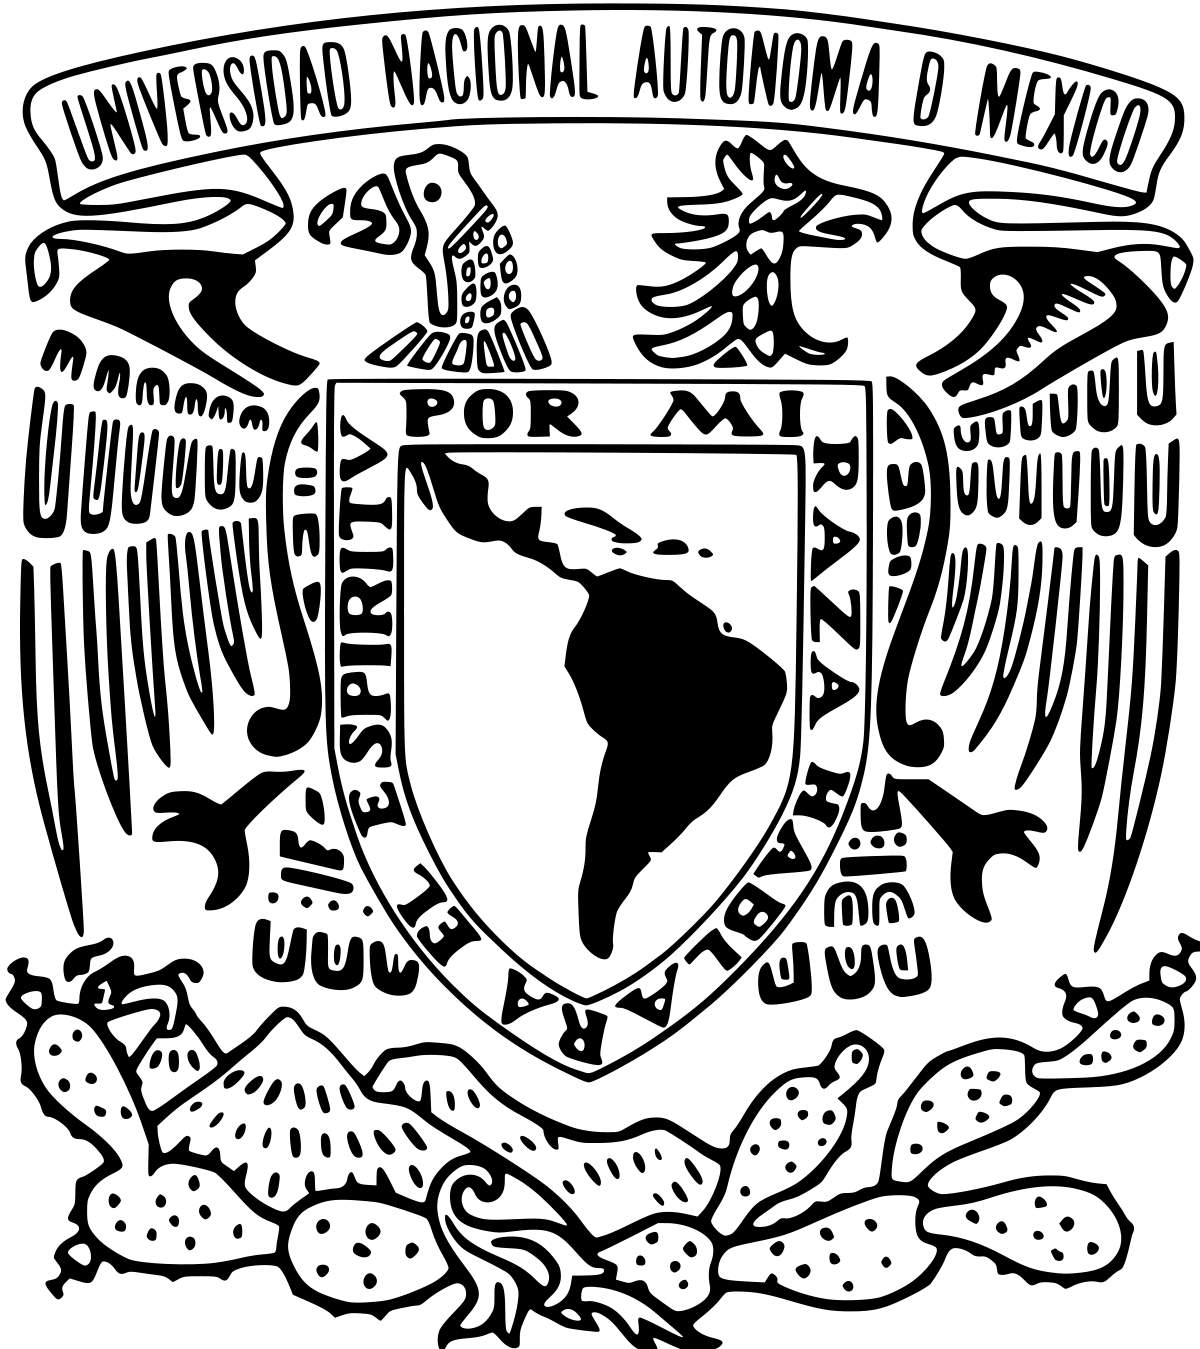
\includegraphics[height = 0.14\textheight]{recursos/Logo_UNAM.png}\par
    	\end{center}
    \end{minipage}\hfill
    \begin{minipage}{10cm}
    	
    \end{minipage}\hfill
    \begin{minipage}{3cm}
    	\begin{center}
    		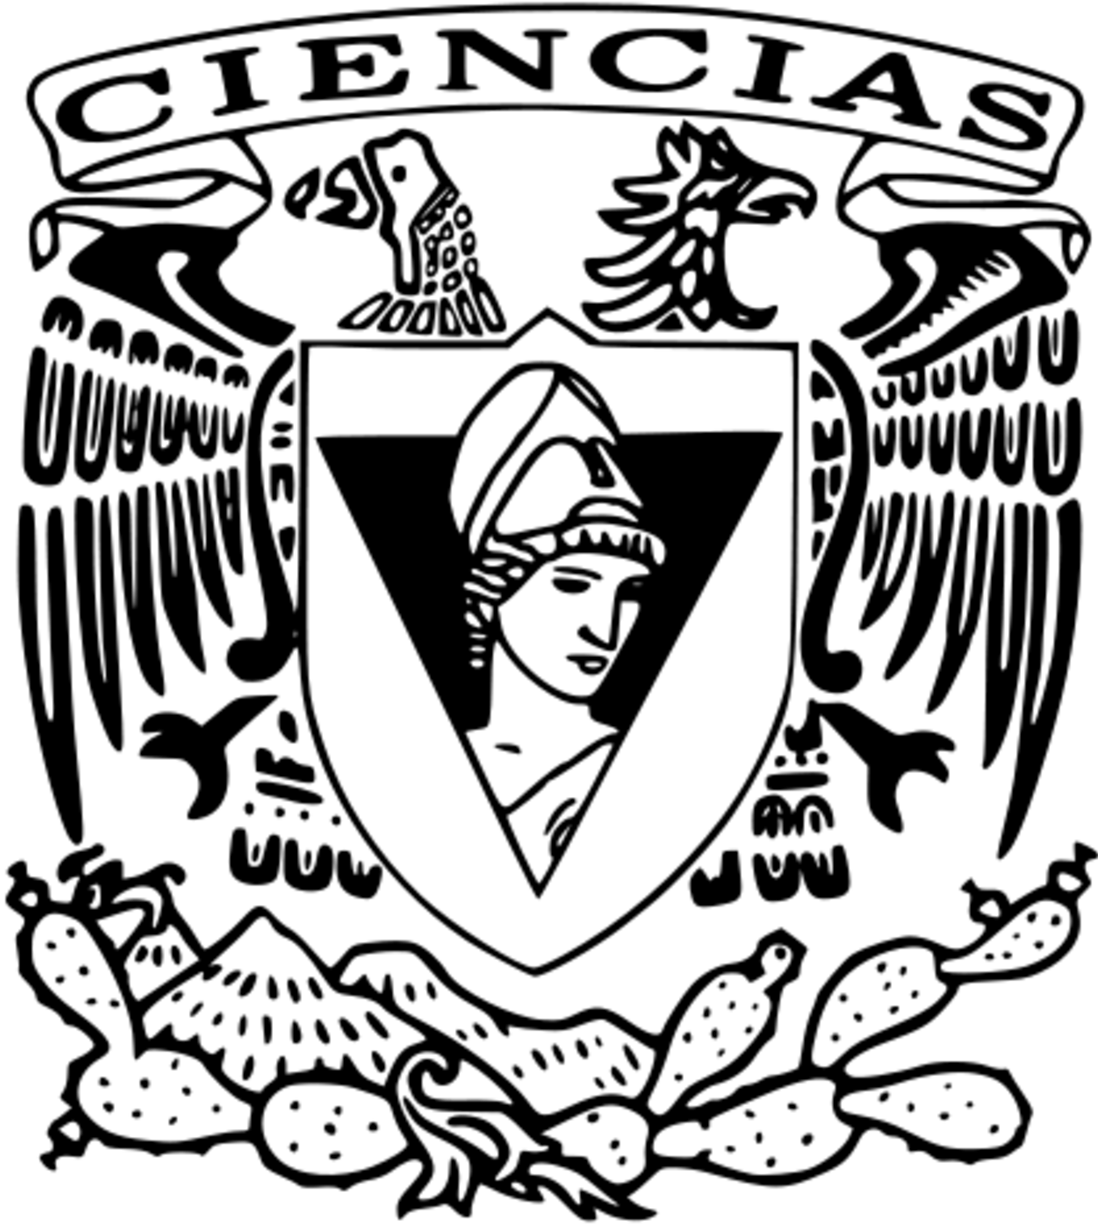
\includegraphics[height = 0.14\textheight]{recursos/Logo_FC.png}\par
    	\end{center}
    \end{minipage}
        \centering
        \vspace{1cm}
        
        {\bfseries\LARGE Universisdad Nacional Autónoma de México \par}
        
        \vspace{1cm}
        {\scshape\Large Facultad de Ciencias \par}
        \vspace{1cm}
        {\scshape\Large Matemáticas para las Ciencias Aplicadas 1 \par}
        \vspace{1cm}
        {\scshape\Large Licenciatura en Ciencias de la Computación \par}
        \vspace{1cm}
        {\scshape\Huge 1ra lista de problemas  \par}
        \vspace{3cm}
        {\itshape\Large Primer Parcial \par}
        \vfill
        {\Large Autores: \par}
        {\Large Ramírez Mendoza Joaquín Rodrigo \par}
        {\Large Villalobos Juárez Gontran Eliut\par}
        {\Large Treviño Puebla Héctor Jerome \par}
        \vfill
        {\Large Agosto 2024 \par}
    \end{titlepage}
% ---Fin de la portada de la portada
    \maketitle

% Introducir aquí sus capítulos
\chapter*{Un balón de futbol americano}
\section*{Un balón de futbol americano}
En este ejercicio se trata de calcular aproximadamente el volumen V de un balón
de football americano profesional suponiendo que su superficie se genera rotando,
alrededor del eje horizontal, una curva y = y (x) que satisface que la longitud del eje
entre las dos puntas del balón es de 28 cm y la circunferencia de la máxima sección
circular transversal al eje mide 53 cm (véase la siguiente figura).

a) Rebane la mitad derecha del balón en 10 cilindros de grosor $\Delta x = 1.4$ cm, de manera
que las rebanadas intersecten el eje x en los valores de la siguiente particiónn del intervalo
$[0, 14]$ 
1) Muestre que la parábola es, aproximadamente, la gráfica de la función
    $$y(x)=-0.043x^2 + 8.4352$$
definida para $-14\leq x\leq 14$


\begin{itemize}
    \item Sabemos que la $\text{Circunferencia}=2\pi r \therefore r=\frac{53}{2\pi}$
    \item la fórmula de las cónicas para la parábola es $y(x)=ax{^2}+bx+c$
    \item sabemos que el radio de la circunferencia del balón es la longitud del radio cuando $x=0$, queremos saber el valor de y para $x=0$
\end{itemize}

\begin{gather*}
\therefore y(0)=\frac{53}{2\pi}=a(0){^2}+b(0)+c=c\\
\Rightarrow c=\frac{53}{2\pi}
\end{gather*}
wTambién conocemos dos puntos que pasan por la ecuación del balón y son los puntos extremos, para encontrar los valores de $a,b$ sustituimos estos valores y resolvemos el sistema de ecuaciones
\begin{gather*}
y(14)=a(14){^2}+b(14)+c\\
y(-14)=a(-14){^2}+b(-14)+c\\
\text{-------------------------------------------------}\\
196a+c=0\\
+196a+c=0\\
\text{----------------------}\\
392a+2c\Rightarrow a=-\frac{2c}{392}=-\frac{c}{196}\\
\therefore y(x)=-\frac{c}{196}x{^2}+c\\
\Rightarrow y(x)=-\frac{\frac{53}{2\pi}}{196}x{^2}+\frac{53}{2\pi}\\
\end{gather*}
Simplificando tenemos que $$y(x)\simeq-0.0430x{^2}+8.4352$$
Podemos expresar la función en términos de $r_0$, de esta manera podemos deducir el dominio de la función.
\begin{gather*}
y(x)=-\frac{c}{196}x{^2}+c\\
y(x)=-\frac{r_{o}}{196}x{^2}+r_{o},\text{donde }r_o=c\\
\text{Igualamos a cero para determinar las raices}\\
-\frac{r_{o}}{196}x{^2}+r_{o}=0\\
-\frac{r_{o}}{196}x{^2}=-r_{o}\\
-r_{0}x{^2}=-r_{0}(196)\\
x{^2}=\frac{-r_{0}(196)}{-r_{0}}\\
x=\pm \sqrt{196}\\
x=\pm 14\\
\therefore-14\leq x\leq 14
\end{gather*}
estos puntos, como habíamos definido antes, son los puntos de corte del centro del balón, solo estamos definiendo, en este caso la mitad de arriba del balón para aproximar su volumen. Esto de ve reflejado con el coeficiente $a$ negativo ($-a$).

2) Muestre que la aproximación del volumen (7) con los 10 cilindros circunscritos de grosor $\Delta x = 1.4 cm$ y radios $y(x_{k})$ cm para $k = 0, 1, 2, . . . , 9$ es:
$$V\simeq 2 \; x \;1825.5143=3651.0286 cm^3$$

La aproximación del volumen para el balón de futbol es: \begin{gather*}
    \sum_{k=0}^{9}V_{k}\\
    \text{donde: } V_{k}=\pi*r_{k}{^2}*\Delta h\\\Delta h=1.4,\text{la altura de cada cilindro}\\
    \end{gather*}
    el valor de correspondencia para cada $x_{k}=\Delta h*k$, la hayamos sustituyendo en la fórmula $r_{k}=y(x_{k})=y(x)\simeq-0.0430x_{k}{^2}+8.4352$.
Decimos que$$\sum_{k=0}^{9}V_{k}=\sum_{k=0}^{9}\pi*r_{k}{^2}\Delta h$$
Podemos decir que $\pi$ y $\Delta h$ son siempre constantes en la suma, por lo tanto podemos factorizar:

\begin{gather*}
=\pi \Delta h\sum_{k=0}^{9}r_{k}\\
=\pi \Delta h\sum_{k=0}^{9}(-0.0430x_{k}{^2}+8.4352){^2}
\end{gather*}

\begin{table}[!hbt]
    \begin{center}
    \begin{tabular}{| c | c | c | c | c | }
    \hline
    K & $\Delta h \cdot j$ & $y(x_{k})$ & $y(x_{k})^{2}$ & $\Delta h*\pi*y(x_{k}^2)$ \\ \hline
    0 & 0 & 8.4352 & 71.15259904 & 312.9462072 \\
    1 & 1.4 & 8.35092 & 69.73786485 & 306.7238667 \\
    2 & 2.8 & 8.09808 & 65.57889969 & 288.4317398 \\
    3 & 4.2 & 7.67668 & 58.93141582 & 259.1945103 \\
    4 & 5.6 & 7.08672 & 50.22160036 & 220.8866516 \\
    5 & 7 & 6.3282 & 40.04611524 & 176.1324259  \\
    6 & 8.4 & 5.40112 & 29.17209725 & 128.305885 \\
    7 & 9.8 & 4.30548 & 18.53715803 & 81.53086994  \\
    8 & 11.2 & 3.04128 & 9.249384038 & 40.68101085  \\
    9 & 12.6 & 1.60852 & 2.58733659 & 11.37972729  \\ \hline
\multicolumn{5}{ |r| } {suma $ = 1825.5143\;cm{^3}$}\\
\multicolumn{5}{|r|}{$V \simeq 2 x 1825.5143 = 3651.0286 cm3$}\\ \hline
    \end{tabular}
    \caption{Tabla de suma de los factores $x_k$}
    \label{tab:la suma de los cilindros circunscritos como parabola}
    \end{center}
    \end{table}

    Ya que solo calculamos los radios de la parte derecha del balón y considerando que es simétrico, el volumen de el lado derecho es el mismo que el del lado izquierdo, por lo tanto se multiplica por 2.
Muestre que la aproximación del volumen (7) con los 10 cilindros inscritos de
grosor $\Delta x = 1.4$ cm y radios $y (x_{k})$ cm para $k = 0, 1, . . . , 9$ es:
$$V\simeq 2 \; x \;1825.5143=3651.0286 cm^3$$
La aproximación del volumen para el balón de futbol es: 
\begin{gather*}
    \sum_{k=0}^{9}V_{k}\\
    \text{donde: } V_{k}=\pi*r_{k}{^2}*\Delta h\\\Delta h=1.4,\text{la altura de cada cilindro}\\
\end{gather*}
el valor de correspondencia para cada $x_{k}=\Delta h*k$, la hayamos sustituyendo en la fórmula $r_{k}=y(x_{k})=y(x)\simeq-0.0430x_{k}{^2}+8.4352$.
Decimos que$$\sum_{k=0}^{9}V_{k}=\sum_{k=0}^{9}\pi*r_{k}{^2}\Delta h$$
Podemos decir que $\pi$ y $\Delta h$ son siempre constantes en la suma, por lo tanto podemos factorizar:
\begin{gather*}
=\pi \Delta h\sum_{k=0}^{9}r_{k}\\
=\pi \Delta h\sum_{k=0}^{9}(-0.0430x_{k}{^2}+8.4352){^2}
\end{gather*}
\begin{table}[!hbt]
    \begin{center}
    \begin{tabular}{| c | c | c | c | c | }
    \hline
    K & $\Delta h \cdot j$ & $y(x_{k})$ & $y(x_{k})^{2}$ & $\Delta h*\pi*y(x_{k}^2)$ \\ \hline
    1 & 1.4 & 8.35092 & 69.73786485 & 306.7238667 \\
    2 & 2.8 & 8.09808 & 65.57889969 & 288.4317398 \\
    3 & 4.2 & 7.67668 & 58.93141582 & 259.1945103 \\
    4 & 5.6 & 7.08672 & 50.22160036 & 220.8866516 \\
    5 & 7   & 6.3282  & 40.04611524 & 176.1324259 \\
    6 & 8.4 & 5.40112 & 29.17209725 & 128.305885  \\
    7 & 9.8 & 4.30548 & 18.53715803 & 81.53086994 \\
    8 & 11.2& 3.04128 & 9.249384038 & 40.68101085 \\
    9 & 12.6& 1.60852 & 2.58733659  & 11.37972729 \\
   10 & 14  & 0.0072  & 5.184E-05   & 0.000228005 \\ \hline
\multicolumn{5}{ |r| } {suma $ = 1825.5143\;cm{^3}$}\\
\multicolumn{5}{|r|}{$V \simeq 2 x 1825.5143 = 3651.0286 cm3$}\\ \hline
    \end{tabular}
    \caption{Tabla de suma de los factores $x_k$}
    \label{tab:la suma de los cilindros inscritos}
    \end{center}
    \end{table}

    b) Suponga ahora que la curva $y = y (x)$ es la mitad superior de una elipse con
    centro en el origen, semieje horizontal $a = 14$ cm (sobre el eje x) y semieje vertical
    $$b = 53 2\pi \simeq 8.4352 cm (sobre el eje y).$$
    Partimos de la ecuación simétrica de la parábola.
    $$\frac{x{^2}}{a{^2}}+\frac{y{^2}}{b{^2}}=1$$Definimos los vértices en $v(0,14)$ y $v'(0,-14)$, por definición sabemos que la mitad de la longitud del semieje mayor es $a$, entonces a=14, $b$ es la mitad del semieje menor, el cual es el radio de nuestro balón, $\Rightarrow b=r_{0}=\frac{53}{2\pi}$
    $$\frac{x{^2}}{14{^2}}+\frac{y{^2}}{r_{0}{^2}}=1$$
    Reducimos hasta despejar a y.
    \begin{gather*}
    14{^2}r_{0}{^2}\left( \frac{x{^2}}{14{^2}} +\frac{y{^2}}{r_{0}{^2}}\right)= 1*14{^2}r_{0}{^2}\\
    \frac{14{^2}r_{0}{^2}x{^2}}{14{^2}} +\frac{r_{0}{^2}14{^2}y{^2}}{r_{0}{^2}}=14{^2}r_{0}{^2}\\
    r_{0}x{^2}+14{^2}y{^2}=14{^2}r_{0}{^2}\\
    14{^2}y{^2}=14{^2}r_{0}{^2}-r_{0}x{^2}\\
    y{^2}=\frac{14{^2}r_{0}{^2}-r_{0}x{^2}}{14{^2}}\\
    y{^2}=\frac{r_{0}{^2}}{14{^2}}(14{^2}-x{^2})\\
    y=\pm\sqrt{ \frac{r_{0}{^2}}{14{^2}}(14{^2}-x{^2}) }\\
    y=\frac{r_{0}}{14}*\pm\sqrt{(14{^2}-x{^2})}\\
    y=\frac{r_{0}}{14}*\pm\sqrt{196-x{^2}}
    \end{gather*}
    
    Sustituyendo $r_0=\frac{53}{2\pi}$ tenemos que $$\frac{r_{0}}{14}=\frac{\frac{53}{2\pi}}{14}\simeq 0.6025\therefore y(x)=0.6025\pm \sqrt{ 196-x{^2} }$$
    Podemos observar que $x{^2}$ solo puede valor, máximo 196 ya que la función no está definida para la raíz cuadrada de un número negativo. $\therefore -14\leq x\leq 14$ 
    
    d) Muestre que la aproximación del volumen (7) con los 10 cilindros circunscritos de
    grosor $\Delta x = 1.4 cm$ y radios $y (x_{k})$ cm para$k = 0, 1, 2, . . . , 9$ es:
    $$V \simeq 2 \times 2237.4593 = 4474.9186 cm3$$
    
    Partimos de que 
    $$V_{total}=\sum_{k=0}^{9}V_{k}$$
    donde $V_{k}=$ a cada volumen de disco con índice k y el volumen se traduce como$$V_{k}=\pi*\Delta h*r_{k}{^2}$$
    y el la medida del radio $r_{k}$ para cada cilindro circunscrito es el valor de $y(x_k)$, para $x_{k}=\Delta h*k$
    y $\Delta h$ es la altura correspondiente que es constante en cada cilindro.
    
    Así denotamos que \begin{gather*}
    \sum_{k=0}^{9}V_{k}=\sum_{k=0}^{9}\pi* r_{k}{^2}*\Delta h
    \end{gather*}
    donde $\pi$ y $\Delta h$ son siempre constantes, factorizamos
    \begin{gather*}
    \sum_{k=0}^{9}\pi* r_{k}{^2}*\Delta h
    =\pi \Delta h\sum_{k=0}^{9} r_{k}{^2}\\
    \text{sustituyendo }r_k \text{ por } y(x_{k})\\
    V_{tottal}=\pi \Delta h\sum_{k=0}^{9} y(x_{k}){^2}\\
    =\pi \Delta h\sum_{k=0}^{9} (0.6025 \sqrt{ 196-x_{k}{^2} }){^2}\\
    \end{gather*}
    así conseguimos la suma de los triangulo circunscritos para calcular el Balón de futbol.

    \begin{table}[!hbt]
        \begin{center}
        \begin{tabular}{| c | c | c | c | c | }
        \hline
        K & $\Delta h \cdot j$ & $y(x_{k})$ & $y(x_{k})^{2}$ & $\Delta h*\pi*y(x_{k})^2$ \\ \hline
        0 & 0    & 8.435       & 71.149225  & 312.930636 \\
        1 & 1.4  & 8.39271903  & 70.4377328 & 309.801329  \\
        2 & 2.8  & 8.26457839  & 68.303256  & 300.41341   \\
        3 & 4.2  & 8.04647716  & 64.7457948 & 284.766878  \\
        4 & 5.6  & 7.7308052   & 59.765349  & 262.861734  \\
        5 & 7    & 7.30492428  & 53.3619188 & 234.697977 \\
        6 & 8.4  & 6.748       & 45.535504  & 200.275607  \\
        7 & 9.8  & 6.02379488  & 36.2861048 & 159.594624   \\
        8 & 11.2 & 5.061       & 25.613721  & 112.655029   \\
        9 & 12.6 & 3.67673126  & 13.5183528 & 59.4568208   \\ \hline
    \multicolumn{5}{ |r| } {suma $2237.45404\; cm^3$}\\ \hline
        \end{tabular}
        \caption{Tabla de suma de los factores $x_k$}
        \label{tab:la suma de los cilindros circunscritos interpretados como una elipse}
        \end{center}
        \end{table}
        Como calculamos la mitad del balón, la suma de la parte derecha la multiplicamos por 2
$$\therefore V \simeq 2 \times 2237.4540 = 4474.90809 \;cm3$$
a) Muestre que la aproximación del volumen (7) con los 10 cilindros inscritos de
grosor $\Delta x = 1.4 cm$ y radios $y (xk)$ cm para$k = 1, 2, . . . , 10$ es:
$$V \simeq 2 \Delta 1924.5279 = 3849.0558 cm^3$$
Tenemos  la misma primicia del anterior.
$$V\simeq\pi \Delta h\sum_{k=1}^{10} (0.6025 \sqrt{ 196-x_{k}{^2} }){^2}$$

\begin{table}[!hbt]
    \begin{center}
    \begin{tabular}{| c | c | c | c | c | }
    \hline
    K & $\Delta h \cdot j$ & $y(x_{k})$ & $y(x_{k})^{2}$ & $\Delta h*\pi*y(x_{k})^2$ \\ \hline
    1 & 1.4  &  8.39271903 & 70.4377328 & 309.801329 \\
    2 & 2.8  &  8.26457839 & 68.303256  & 300.41341 \\
    3 & 4.2  &  8.04647716 & 64.7457948 & 284.766878 \\
    4 & 5.6  &  7.7308052  & 59.765349  & 262.861734 \\
    5 & 7    &  7.30492428 & 53.3619188 & 234.697977 \\
    6 & 8.4  &  6.748      & 45.535504  & 200.275607 \\
    7 & 9.8  &  6.02379488 & 36.2861048 & 159.594624 \\
    8 & 11.2 &  5.061      & 25.613721  & 112.655029 \\
    9 & 12.6 &  3.67673126 & 13.5183528 & 59.4568208 \\
   10 & 14   & 0           & 0          & 0          \\ \hline
\multicolumn{5}{ |r| } {suma $1924.52341\; cm^3$}\\\hline
    \end{tabular}
    \caption{Tabla de suma de los factores $x_k$}
    \label{tab:la suma de los cilindros inscritos interpretados como una elipse}
    \end{center}
    \end{table}
    \break
    Como calculamos la mitad del balón, la suma de la parte derecha la multiplicamos por 2.
    $$\therefore V \simeq 2 \times 1924.5279 = 3849.04682 cm3$$

\chapter*{Un jugador de baseball}
\section*{Un jugador de baseball}
    Un jugador de baseball batea la pelota a 3 ft de altura sobre el plato en dirección a la barda del jardín central que está a 400 ft de distancia de home y tiene 10 ft de altura. La pelota sale con rapidez de 115 $\frac{ft}{s}$ y un ángulo de elevación de 50° sobre la horizontal.
    
    1) Sabemos que el vector de movimiento $\vec{v}=115\frac{ft}{s}$ de la pelota se puede descomponer en dos direcciones de velocidad, movimiento rectilíneo y tiro vertical y caída libre ya que su comportamiento es en dos grados de libertad $$r:\left[0,t\right]\rightarrow \mathbb{R}^2_{(x,y)}$$
    $\therefore$ la componente horizontal del  vector de la bola está representada por la formula del mov. rect. uniforme.$x(t)=v_x(t)=v_{0_x}\Rightarrow x(t)-x_{0}=v_{0_x}(t)\therefore x(t)=v_{0_x}(t)$
    Como el movimiento no es recto completamente, si no que tiene un ángulo de inclinación, requerimos del coseno para calcular la fracción de la velocidad que le corresponde. $$\vec{\|vx\|}=\vec{\|v\|}cos\;\theta = 115cos\;50 = 73.91\frac{ft}{s}$$
    2) La componente vertical del vector resultante está representada por la caída libre, la cual denotamos como $v(t)=gt$.
    El área bajo la recta de velocidad respecto al tiempo representa el desplazamiento del objeto $$\therefore y(t)-y(0)=\frac{1}{2}gt^2$$
    como el movimiento de caída crece un lapso de tiempo y luego decrece hasta tocar el suelo nuestra aceleración es negativa y, además, consideremos que el movimiento empieza a una distancia distinta de cero.$$y(t)-y(0)=v_{0_y}t-\frac{1}{2}gt^2$$ tomando en cuenta que la gravedad es de $32\frac{ft}{s^2}$ $$\Rightarrow y(t)=y(0)+v_{0_y}t-\frac{1}{2}gt^2$$ donde $v_{0_y}$ representa la velocidad respecto de la componente en y, $$\therefore \vec{\|v_y\|}=115 sen\theta 50=89.09\frac{ft}{s}$$, sustituyendo tenemos$$y(t)=3+89.09\frac{ft}{s}t-16t^2$$ donde 3 es la altura en pies donde el bat impacta con la pelota.
    
    \vspace{5mm} %5mm vertical space        
    
    3) Sabemos que $x(t)$ es la fórmula de la distancia que tomará la bola respecto a cada segundo que dura el movimiento. Queremos averiguar cual sería el tiempo en el que la pelota está a 400 metros del bateador para poder determinar si la pelota sobrepasa la barrera
    $$x(t)=73.91\frac{ft}{s}t=400ft\therefore t=\frac{400ft}{73.91\frac{ft}{s}}=5.4119s$$
    La pelota tarda $5.4119s$ en llegar a los $400 ft$ de distancia.
    Ahora, para saber la posición de la pelota en ese tiempo tenemos que sustituir el valor del tiempo en la fórmula que nos dice a que altura llega la bola respecto a su desplazamiento.
    $$y(5.4119)=3+89.09\frac{ft}{s}(5.4119s)-16(5.4119s)^2$$
        $$y(5.4119) \simeq 11.1156ft$$
    Concluimos que la pelota supera la barrera de $10ft$ de altura que está a $400 ft$ de distancia ya que la pelota en ese mismo instante se encuentra a una altura superior que el de la barrera.
    
    \vspace{5mm} %5mm vertical space        
    
    Consideremos que la bola choca con un obstáculo a $5ft$ de altura después de pasar la barrera, lo primero que queremos saber es cuando $y(t)=5$
    \begin{gather*}
        y(t)=5=y(t)=3+89.09\frac{ft}{s}t-16t^2\\
        2=88.0951t-16t^2\\
        t=(88.0951-16t)t\\
        t_1=2\\
        t_2:(88.0951-16t_2)=2\\
        -16t_2=-86.0951\\
        t_2=\frac{-86.0951}{-16}\\
        t_2=5.4839s
    \end{gather*}
    Tengamos en cuenta el movimiento parabólico que tiene la pelota, entonces pasa en 2 tiempos diferentes a los $5 fts$, considerando el mayor de ellos (parte final del movimiento), tenemos que, para saber la posición a la que se encontraba la bola en ese tiempo usaremos la formula de posición $x(t)$.
    \begin{gather*}
        x(t)=73.9206t\\
        x(5.4839)=73.9206\frac{ft}{s}(5.4839s)\\
        x(5.4839)\simeq405.314ft
    \end{gather*}
    $\therefore$ Concluimos que el movimiento termina, o por lo menos no está definido después de $5.4839s$ en la distancia max. de $405.314ft$.
    
    \vspace{5mm} %5mm vertical space        
    
    c) Para calcular el valor máximo de altura a la que se encuentra la bola en el movimiento tenemos que hacer uso de la primer derivada de la fórmula $y(t)$ que representa la posición de altura para cada valor del tiempo.
    \begin{gather*}
        y'(t)=88.0951t-32t\\
        y'(t)=0=88.0951t-32t\\
        -32t=-88.0951\\
        t=\frac{-88.0951}{-32}\\
        t\simeq 2.7529s
    \end{gather*}
    $t\simeq 2.7529s$ es el valor aproximado del tiempo en el que se encuentra a la altura máxima, este valor lo sustituimos en la ecuación $y(t)$ para saber cual es la posición en ese tiempo.
    \begin{gather*}
        y(2.7529s)=3+89.09\frac{ft}{s}(2.7529s)-16(2.7529s)^2
        y(2.7529s)\simeq 124.2617ft
    \end{gather*}

    \begin{center}
        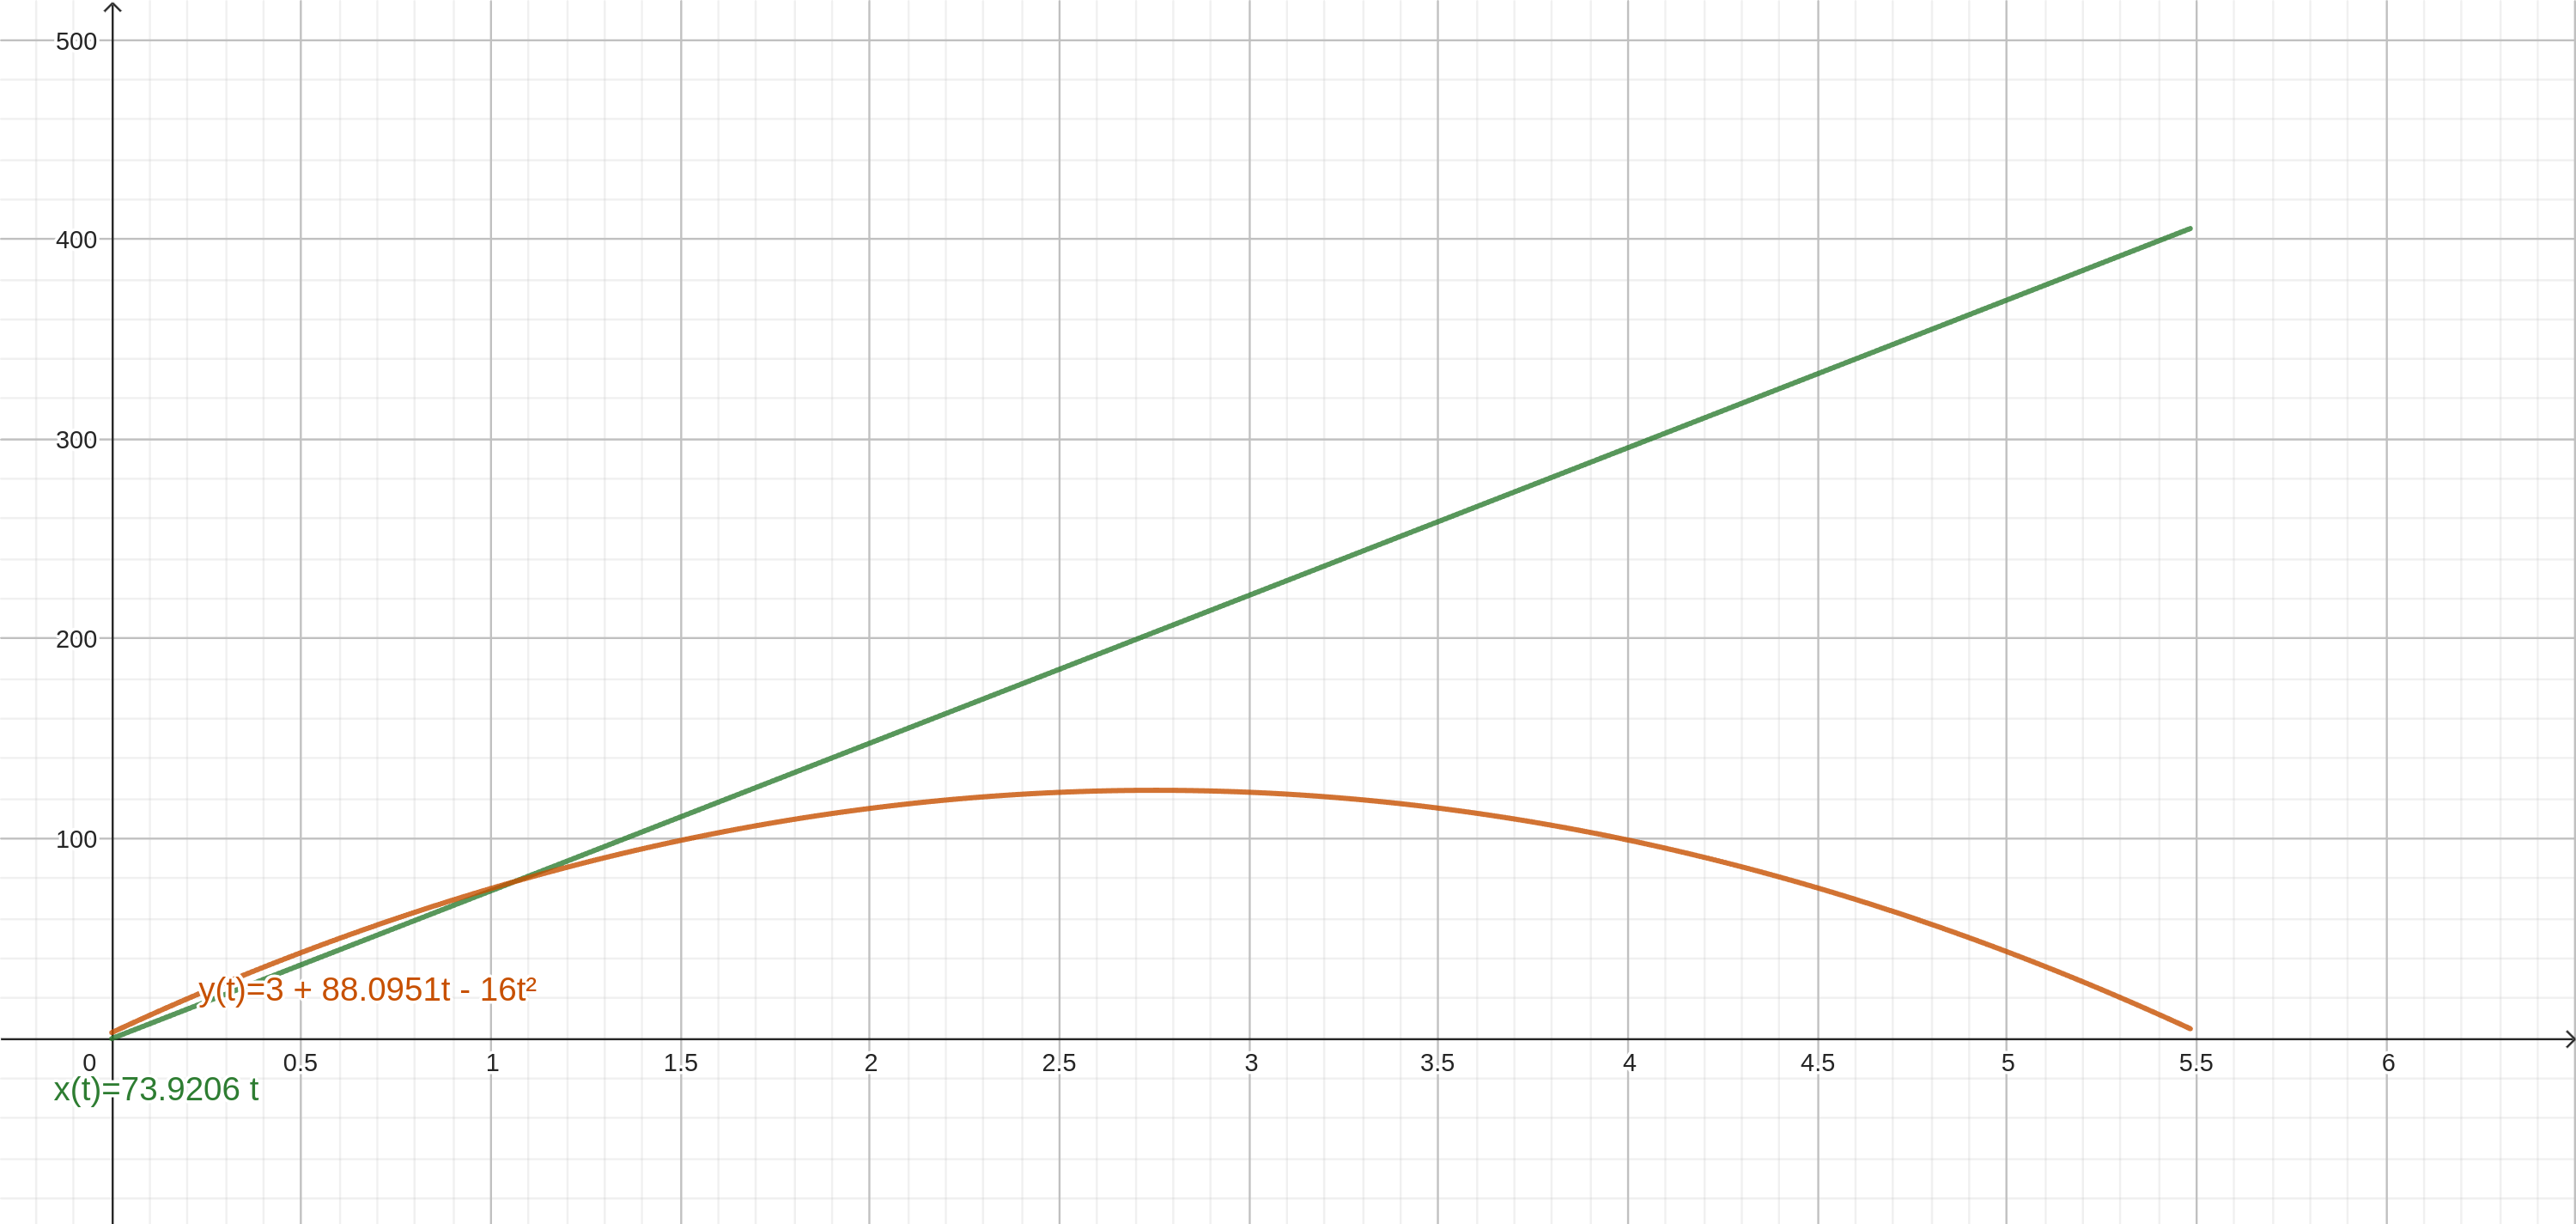
\includegraphics[height = 0.3\textheight]{recursos/geogebra-export(1).png}\par
    \end{center}
    Trayectoria    
    \begin{center}
        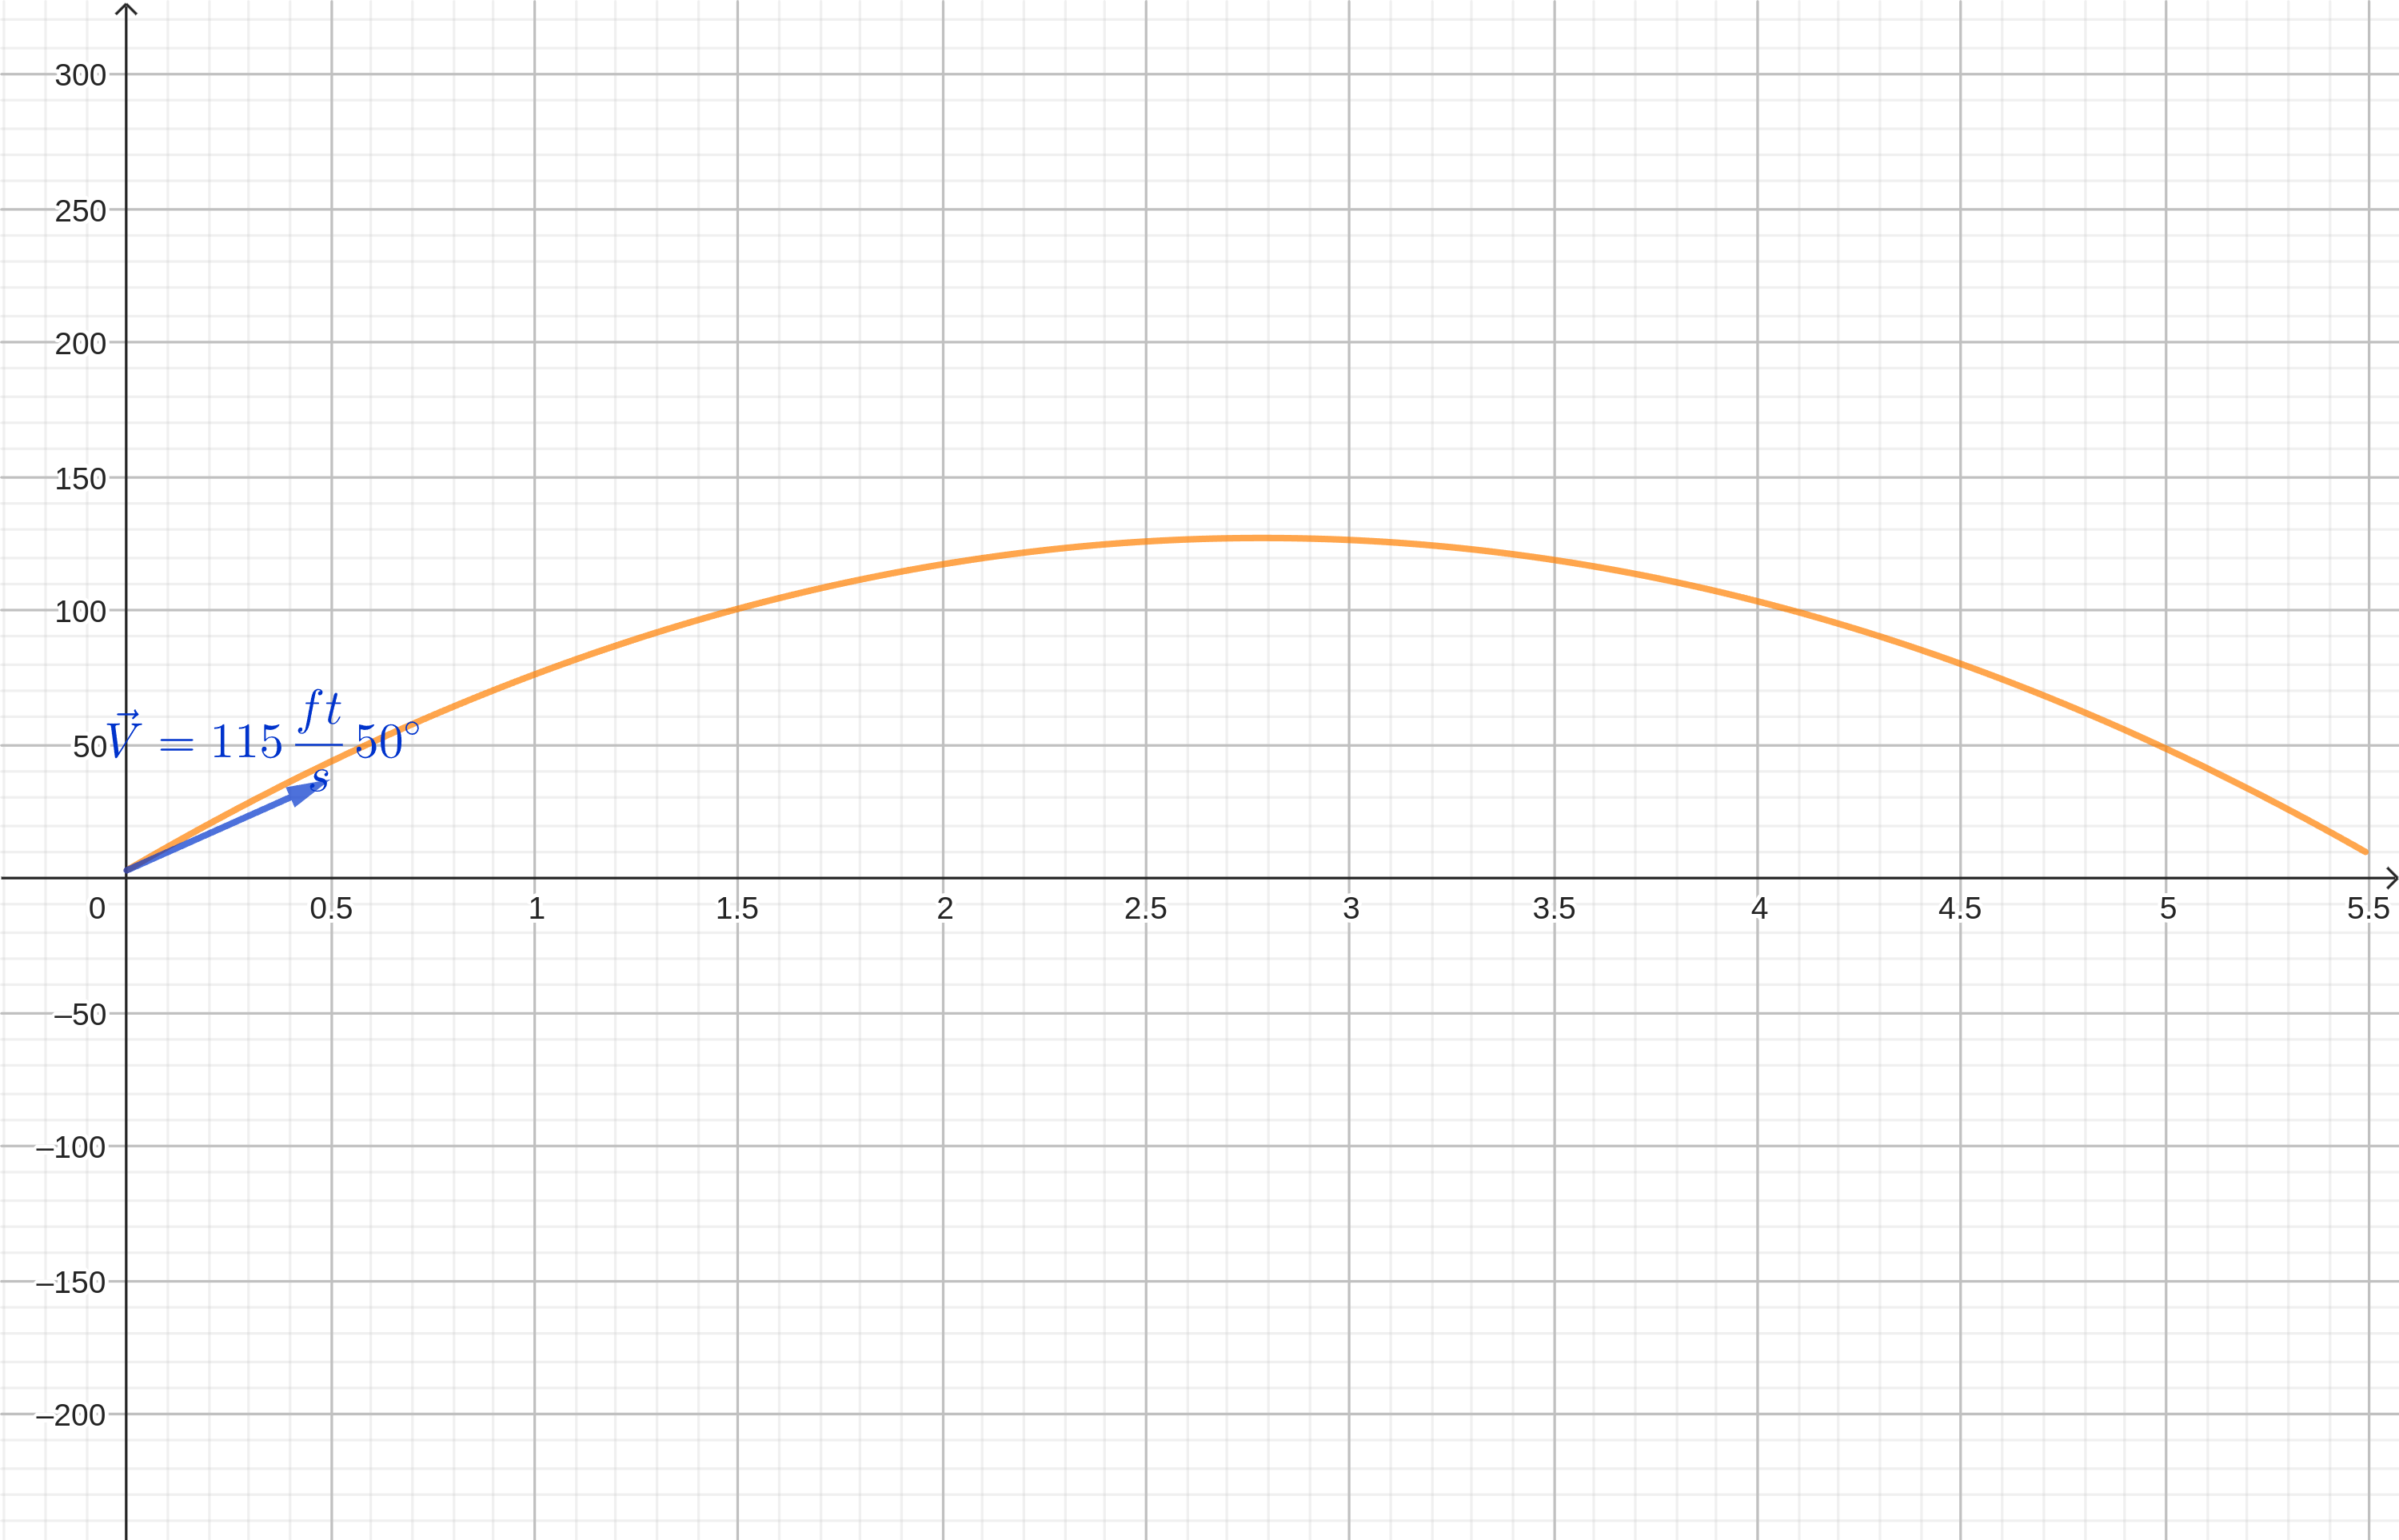
\includegraphics[height = 0.3\textheight]{recursos/geogebra-export(2).png}\par
    \end{center}

\chapter*{Ejercicio 9}
\section*{Pista de atletismo}
a)Mostrar que es posible construir una pista de un cuarto de milla alrededor del
campo de football. (Se sugiere calcular la longitud de la pista más corta que podría
construirse alrededor del campo).

\vspace{0.1cm}

La pista se compone de dos secciones, la sección uno que serían las dos partes rectas y los dos semicírculos. La longitud mínima de las rectas de la pista deben medir lo mismo que el largo de la cancha que es $360ft$, por otra parte, ambos semicírculos, el diámetro mínimo lo consideramos como la anchura de la cancha que es de $160ft$
Sabemos que la circunferencia de un círculo se obtiene con la fórmula $C=\pi d$ donde $d$ es el diámetro.
Entonces, para poder construir la pista con la minima distancia es necesario sumar las dos longitudes a lo largo de la pista más la circunferencia de los dos semicírculos.
$$\Rightarrow L=\pi \cdot d + 2\cdot 360$$
Podemos poner la formula completa ya que los dos semicírculos son iguales y forman un circulo completo de diámetro $160ft$.
Sustituyendo: 
\begin{gather*}
    L=\pi\cdot160ft+\cdot360ft\\
    L\simeq 1222.6548ft\\
\end{gather*}
Podemos notar que el valor dado para construirla pista con la longitud minima constituida por dos semicírculos y dos lados rectos es menor al requerido $1222.6548ft<1320ft$.
\vspace{0.2cm}

b) Sea L la longitud, en pies, de una de las partes rectas de la pista y sea x la distancia, en pies, entre la línea lateral del campo y una de las partes rectas de la pista. Muestre que L como función de x viene dada por:
$$L(x) = 660 - 80 \pi - \pi x$$

y grafique esta regla de correspondencia para $0 \leq x \leq 20$.
\vspace{0.2cm}

Para expresar L en función de x $L(x)$ aumentamos en x el diámetro de los semicírculos de la función de tal manera que: diámetro $$=160 + x$$
Ahora calculamos la circunferencia  $c=\pi*diametro\therefore c=\pi*(160+x)$

Sea $L$ la longitud de los lados rectos para las cuales queremos expresar la variabilidad de su comportamiento en función de $x$.
Entonces queremos saber en que x el valor será de la pista será $1320fts$ en la suma de las longitudes.
\begin{gather*}
    (160ft+x)\pi + 2L = 1320ft\\
    \pi\cdot160ft+\pi\cdot x + 2L = 1320ft\\
    2L = 1320ft - 160\pi ft -\pi x\\
    L=\frac{1320ft - 160\pi ft -\pi x}{2}\\
    L=660-80\pi - \pi x
\end{gather*}

$$\therefore L(x)=660 - 80\pi-\pi x$$

\begin{center}
        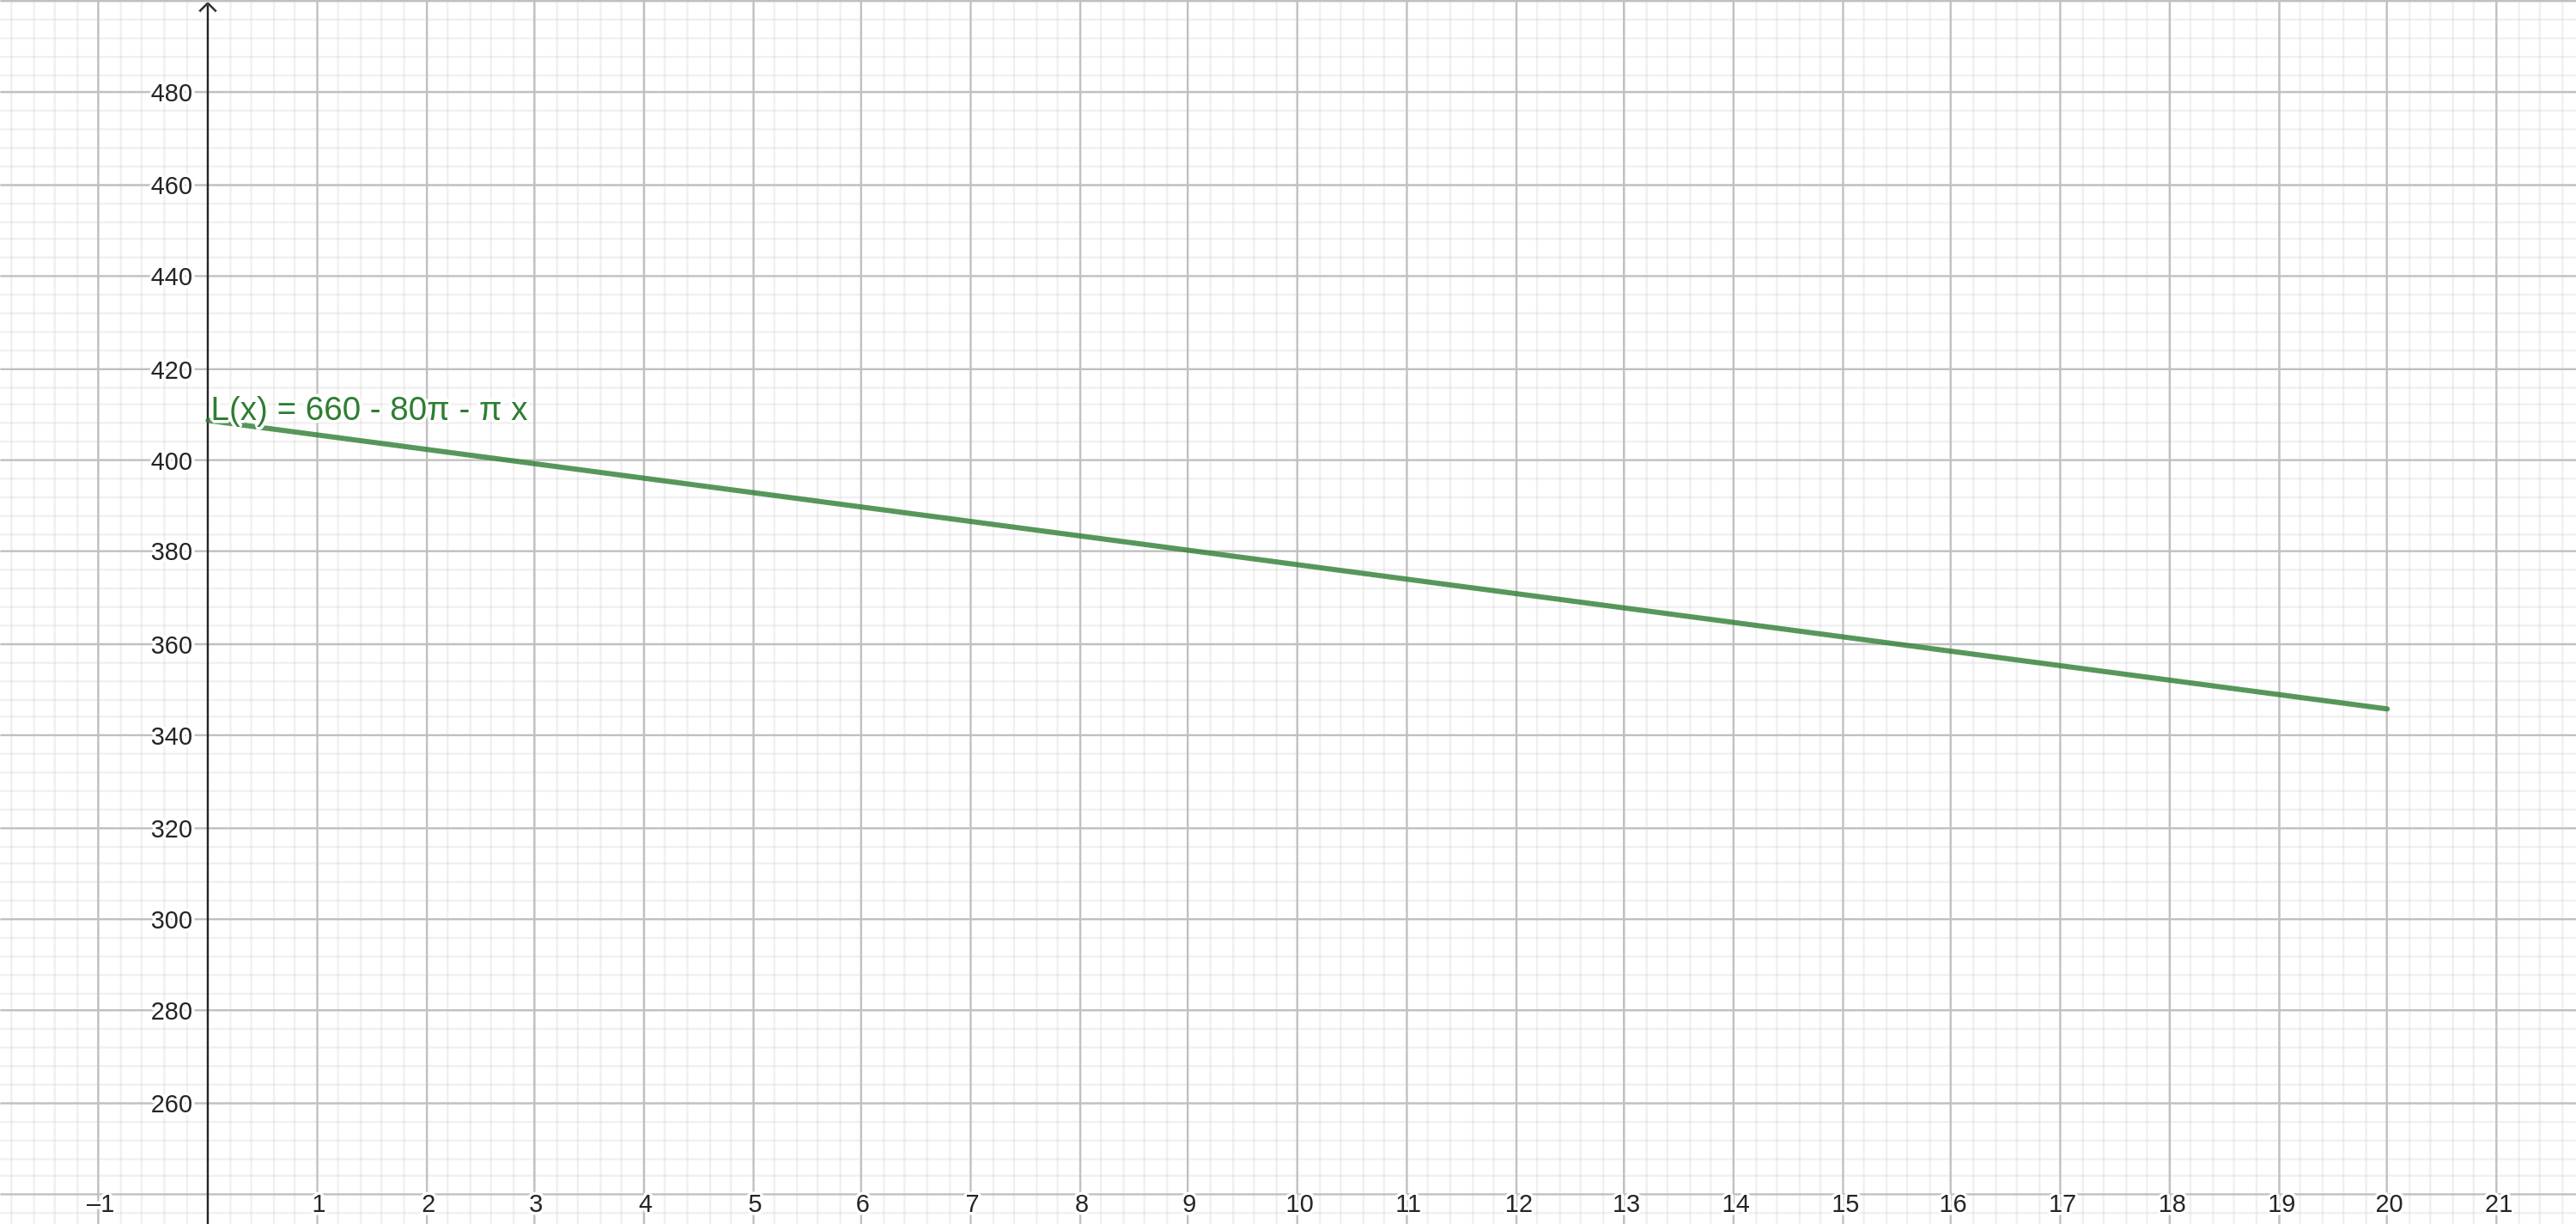
\includegraphics[height = 0.3\textheight]{recursos/geogebra-export.png}\par
\end{center}


Con base en esta
gráfica:

1) Estime la mínima longitud de la parte recta de la pista y, luego, muestre que el valor de x para el que ésta ocurre es aproximadamente 15.49 ft.

Tomando en cuenta que la longitud mínima que puede tomar la pista es de 360 debido a que es la misma longitud que mide el campo de football, queremos saber el valor de separación entre el campo y la pista para que la longitud total de la pista sea $\frac{1}{4}$ de milla = $1320ft$

\begin{gather*}
    360=660-80\pi-\pi x\\
    360-660+80\pi=-\pi x\\
    \frac{360-660+80\pi}{-\pi}=x\\
    \therefore x\simeq 15.49ft
\end{gather*}

$15.49ft$ debe ser la medida aproximada de la distancia entre la pista y el campo para que la pista tenga una Longitud total de $1320ft$.
\vspace*{0.2cm}


2) Estime la máxima longitud de la parte recta de la pista y luego, muestre que el valor de L para el que ésta ocurre es aproximadamente 408.67 ft.

El máximo valor de de la longitud de la parte recta debe ser cuando no hay separación entre el campo de fútbol y la pista, por tanto, debemos sustituir para $ L(0)$.
\begin{gather*}
    L(0)=660 - 20\pi-\pi(0)\\
    L(0)\simeq 408.67ft
\end{gather*}

$\therefore$ La longitud máxima de la parte recta de la pista debe medir $408.67ft$ para que la longitud total de la pista sea de $\frac{1}{4}$ de milla = $1320 fts$
\chapter*{Ejercicio 11}
\section*{Caja con tapa superior}

11. De un pedazo rectangular de cartón de 6 ft pot 10 ft se va a fabricar \textbf{\textit{una caja con tapa superior}} doblando a lo largo de las líneas punteadas, cortando cuatro cuadrados del mismo tamaño (véase la figura 1) y plegando dentro de la caja las dos pestañas extras.
\newline
\begin{center}
     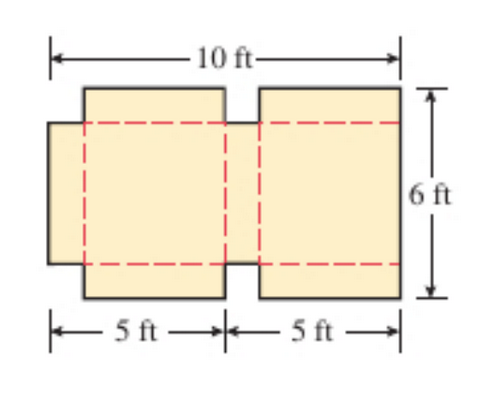
\includegraphics[width=5cm]{recursos/Caja_doc_tarea.png}\par
\end{center}

\textbf{a)} Hallar una fórmula que exprese el volumen V de la caja como función de la longitud x de los lados de los cuadrados que se cortan.\\
\[
V = (largo)(ancho)(alto)
\]
\begin{itemize}
        \item $largo = 5 -x$
        \item $ancho = 6 -2x$
        \item $alto = x$
    \end{itemize}
\[
V(x) = (5-x)(6-2x)(x)
\]
\[
V(x) = (30-10x-6x+2x^{2})(x)
\]
\[
V(x) = (30-16x+2x^{2})(x)
\]
\[
V(x) = 2x^{3}-16x^{2}+30x 
\]
\begin{center}
    Fórmula para el volumen en función de x: \underline{ $V(x) = 2x^{3}-16x^{2}+30x $ ft³} 
\end{center} 

\textbf{b)} Describa, mediante una desigualdad que acote los posibles valores de x, el dominio de definición de a función V = V (x) del inciso anterior. \\
\newline
Dominio Natural de V(x): $R$ \\
Dominio de Definición de V(x): $0 < x < 3$
\begin{itemize}
    \item x debe ser mayor de 0 para que pueda doblar y formar la caja. $x > 0$
    \item x debe ser menor de 3 o no podría haber 2x en el lado de 6 ft. $x < 3$
\end{itemize}
\begin{center}
    Dom. Definición: \underline{$0 < x < 3$}
\end{center}



\textbf{c)} Usar la gráfica de V = V(x) para dar valores aproximados de las dmonsiones de la caja de máximo volumen.
\begin{center}
     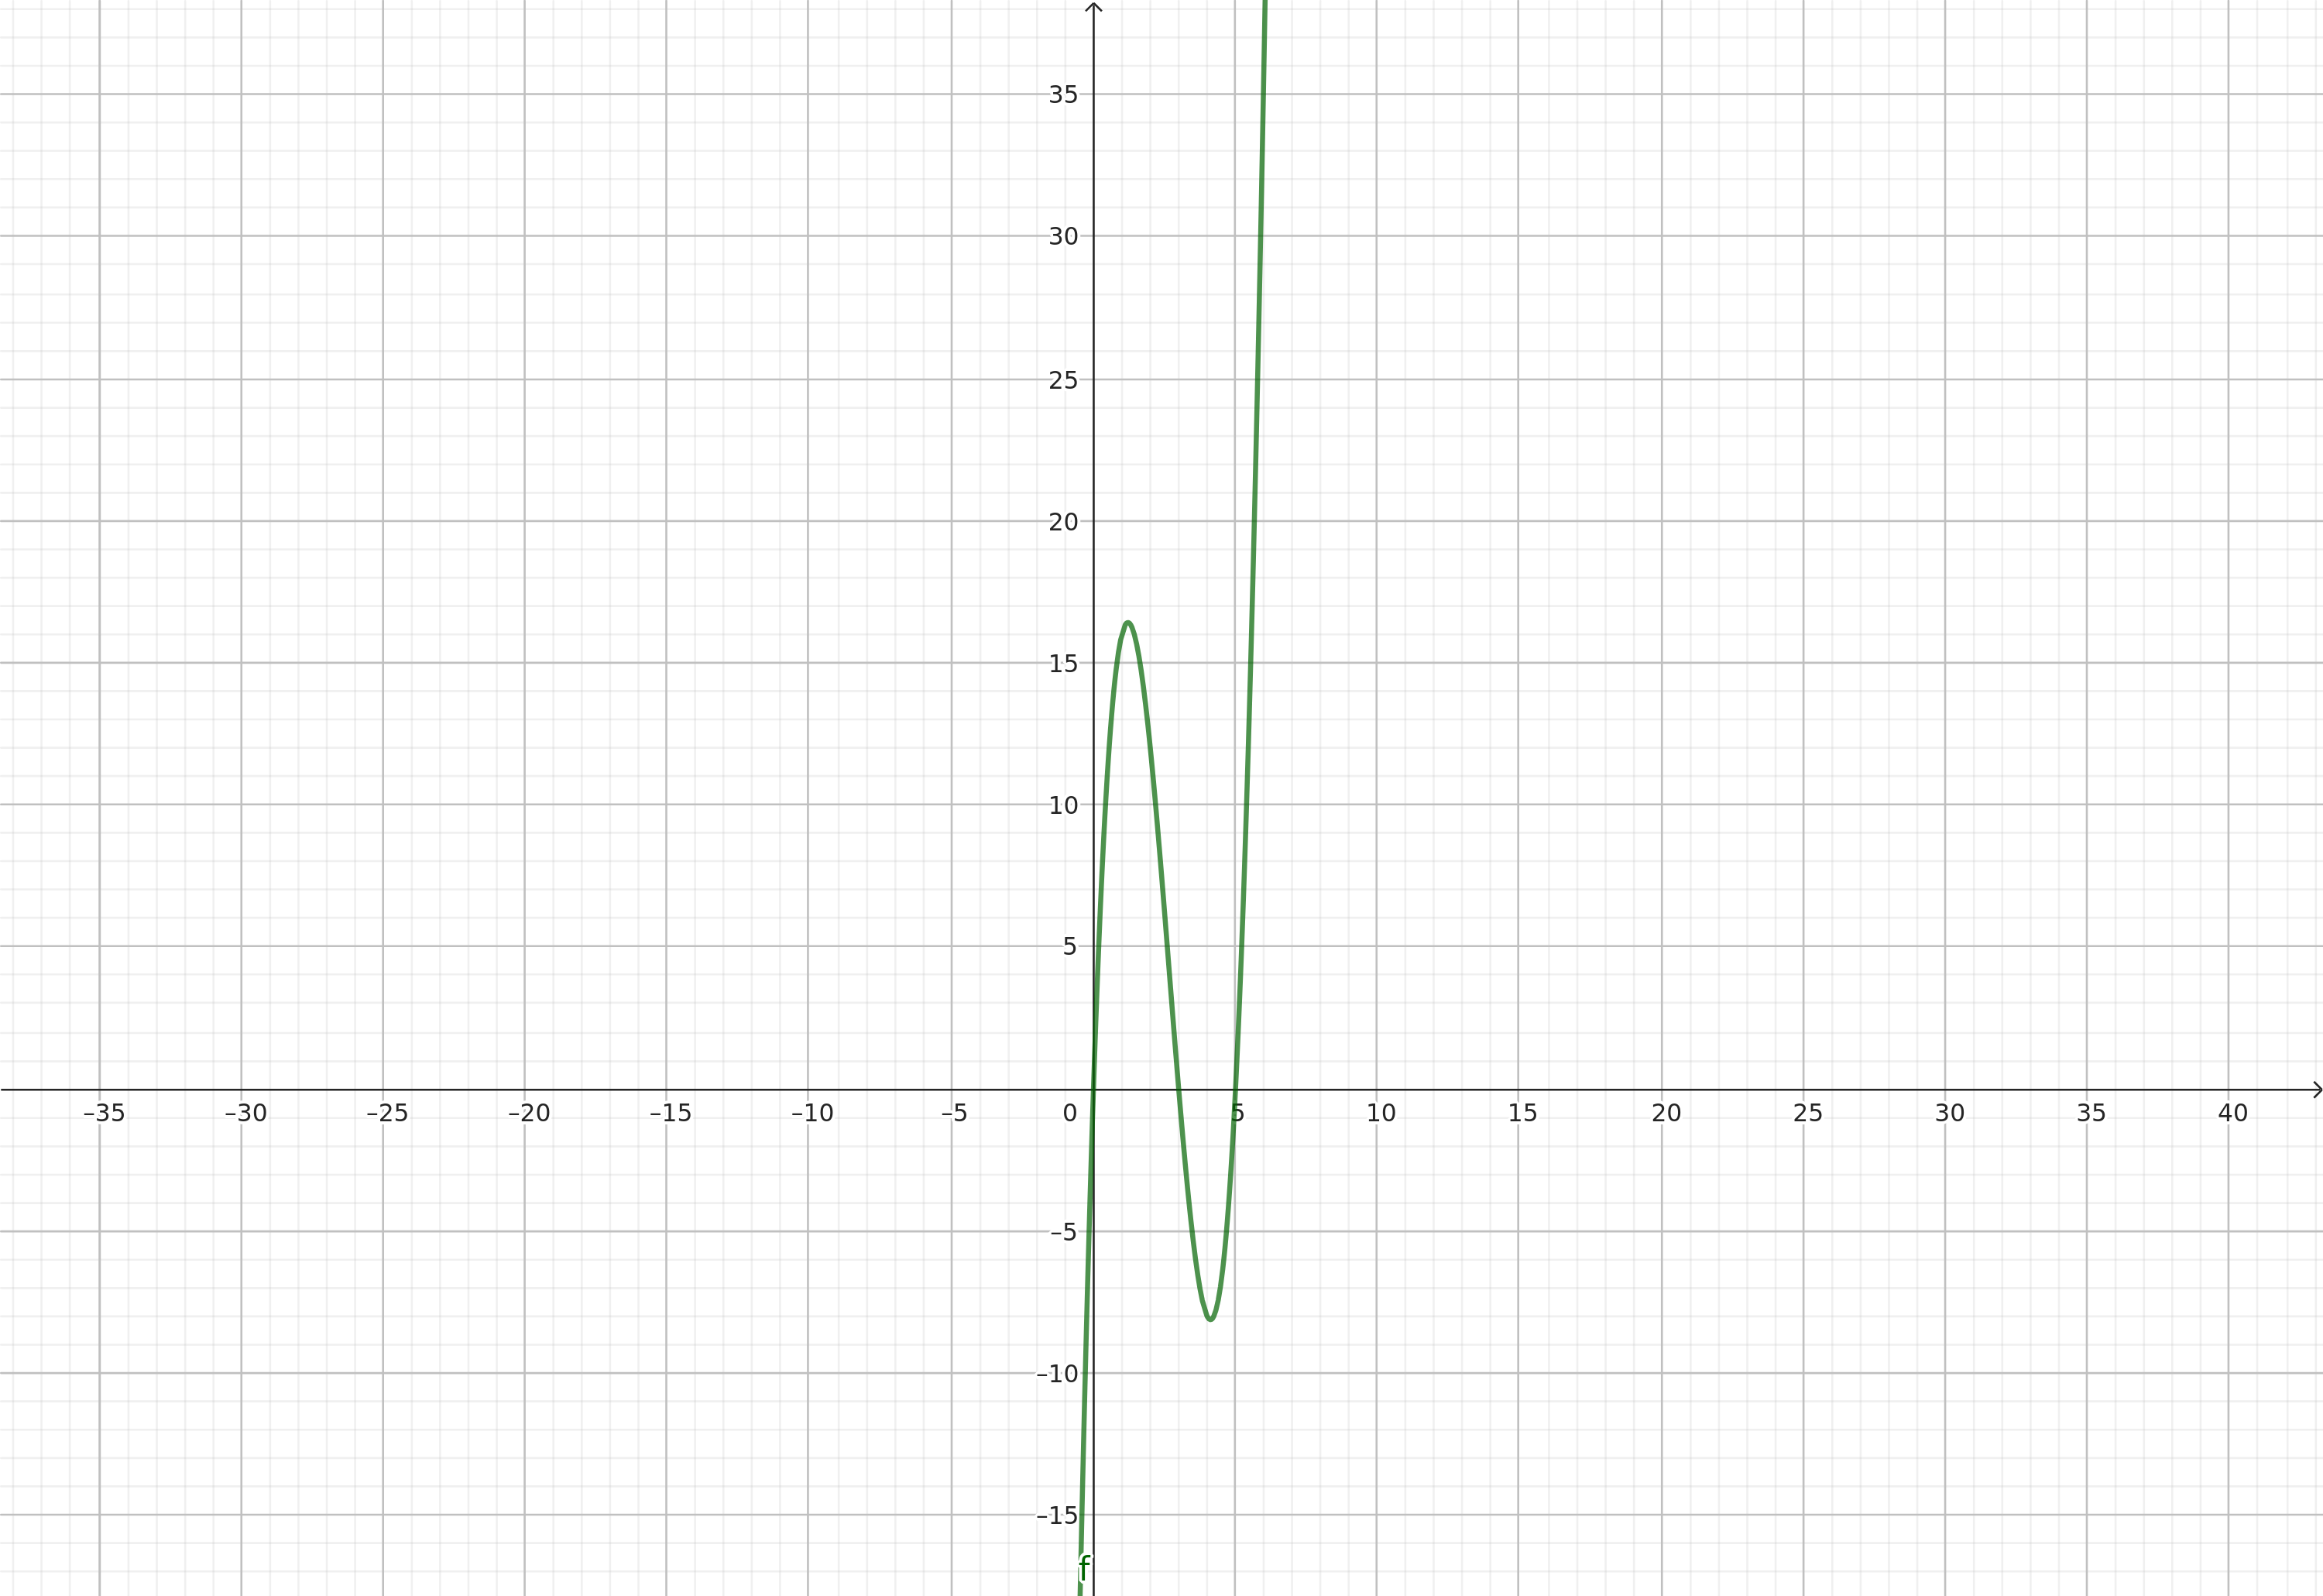
\includegraphics[width=9cm]{recursos/Grafic_caja.png}\par
     Gráfica de $V(x) = 2x^{3}-16x^{2}+30x $
\end{center}
\par
\begin{center}
     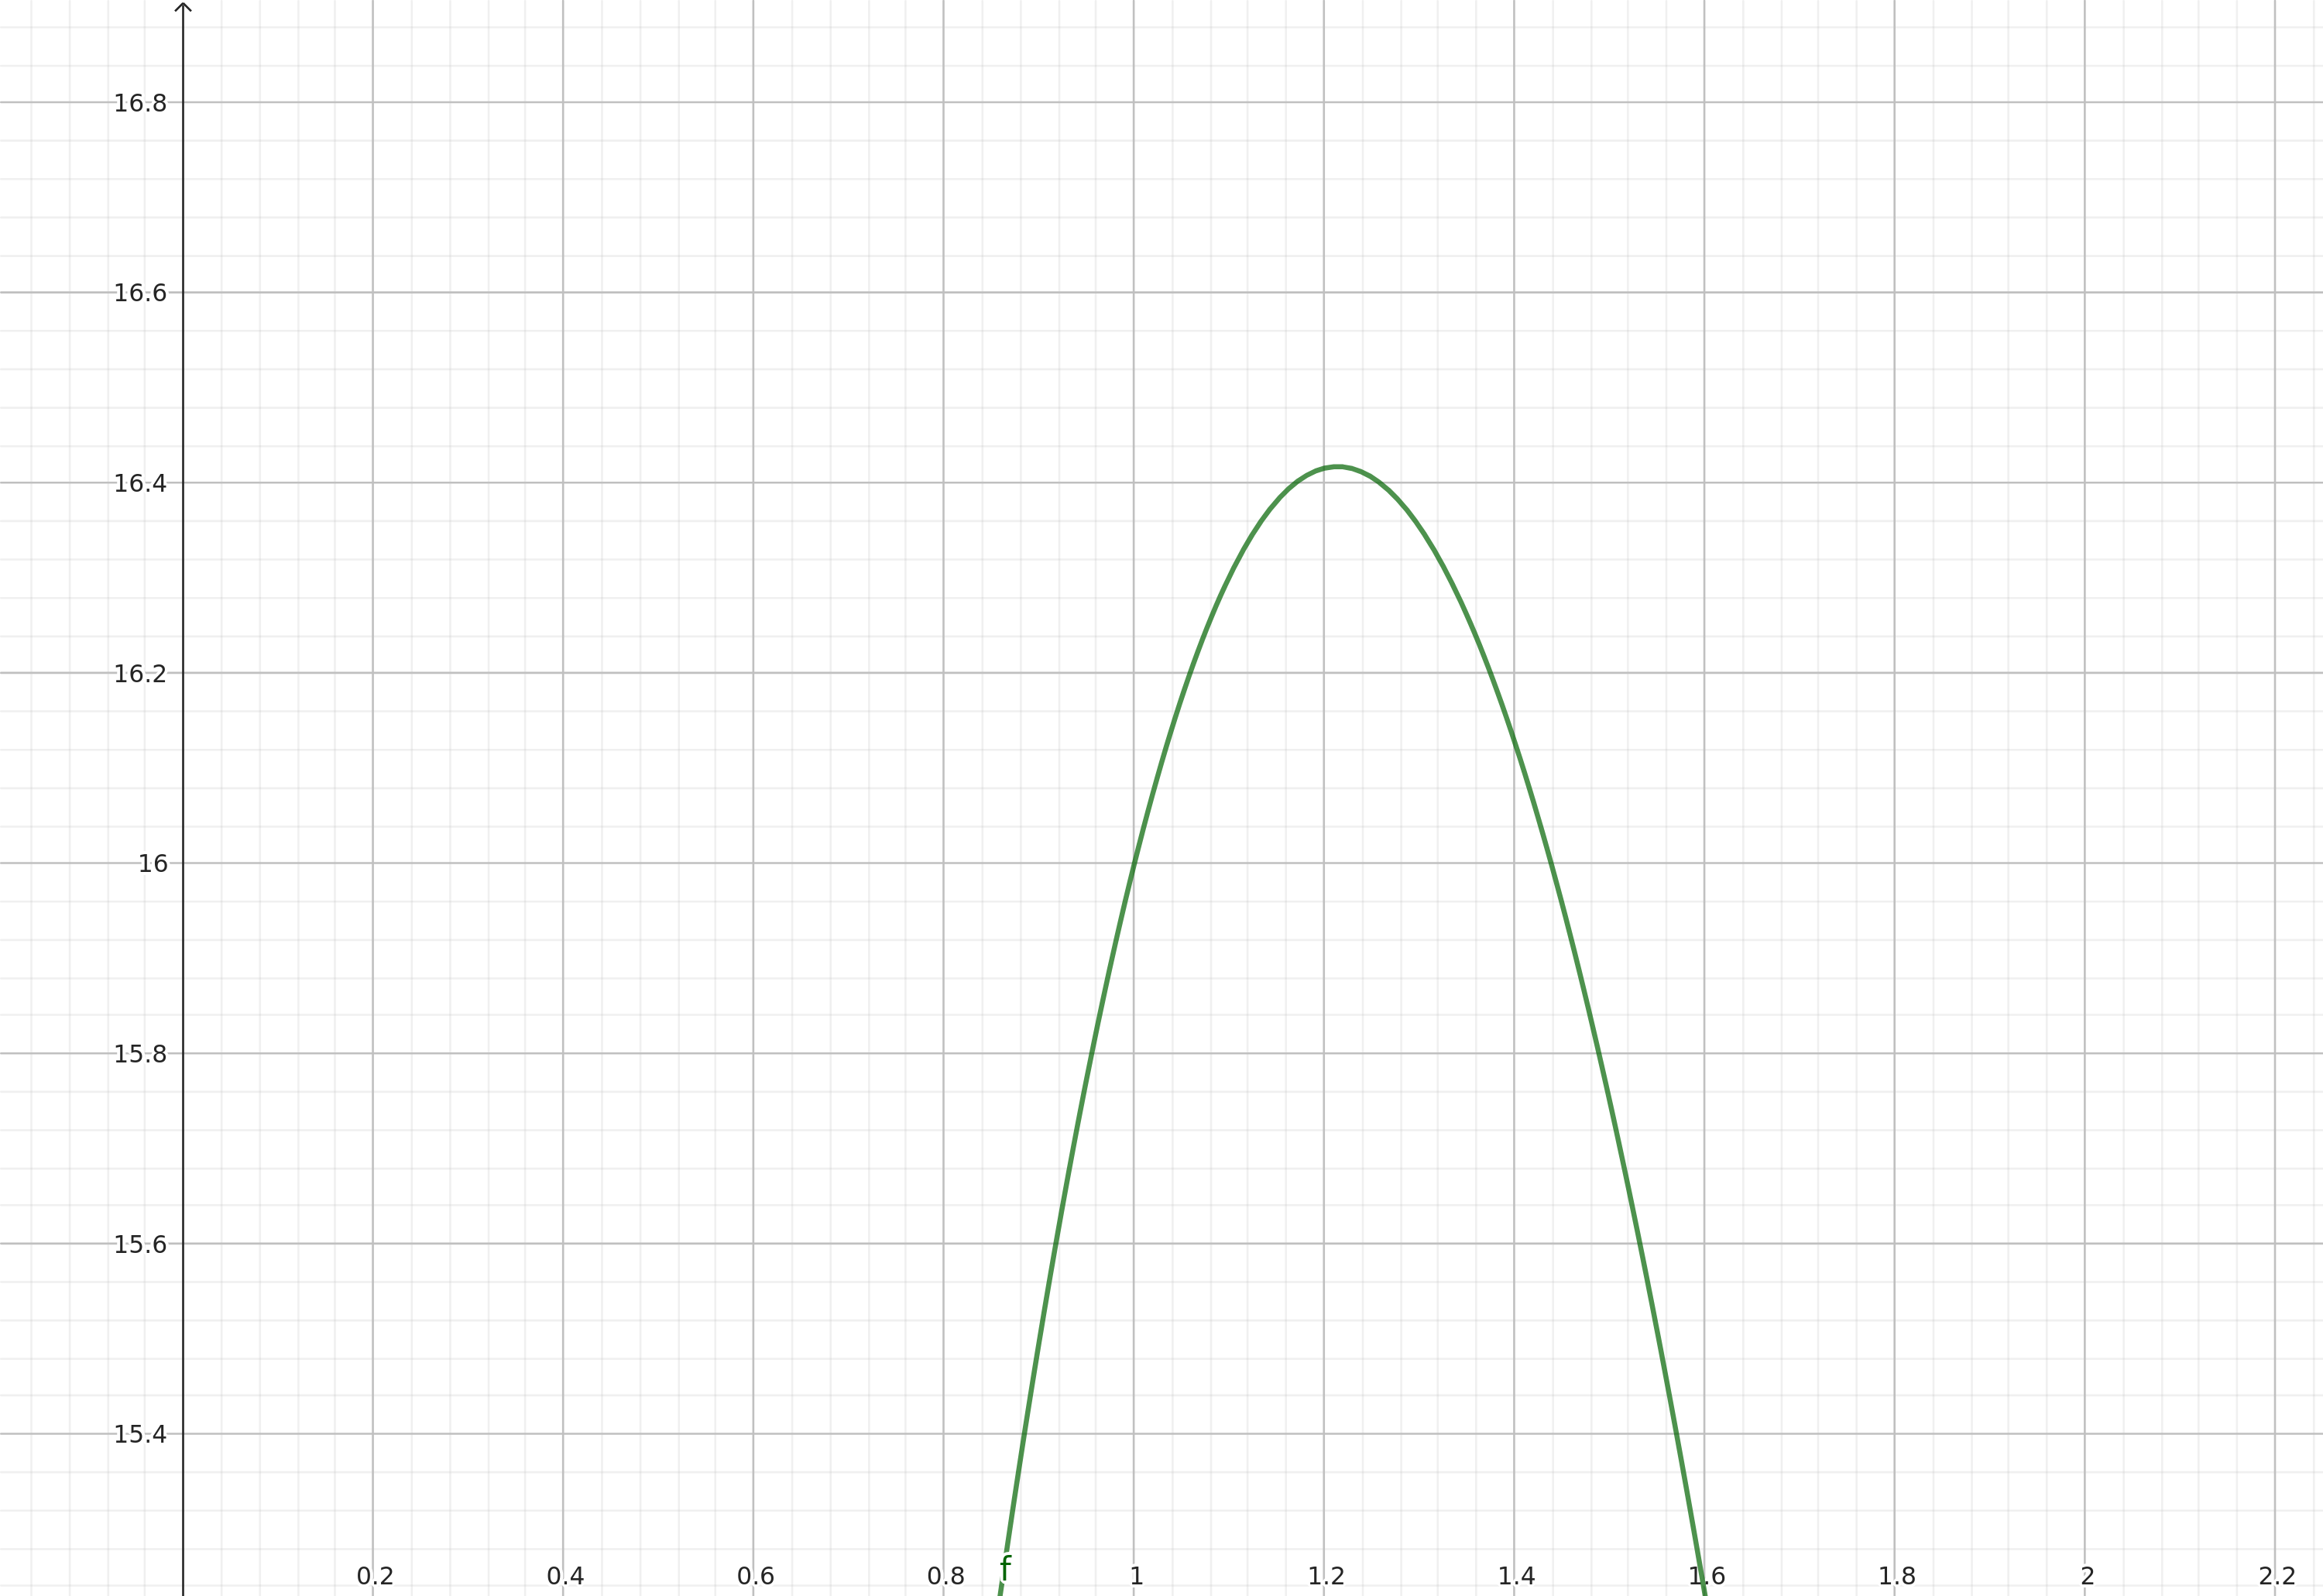
\includegraphics[width=9cm]{recursos/Problema_caja3.png}\par
     Valores Máximos que toma el volumen: \\
     Cuando $x$ se aproxima a 1.2137\\
     $Vol. Max. \approx 16.4176  ft^{3}$
\end{center}

\chapter*{title}
\section{Modelo de Crecimiento Poblacional}

    **Introducción**

    Se presenta un modelo matemático para describir el crecimiento de una población de borregas, dado por la siguiente función:
    * $N(t)$ representa el número de borregas en el tiempo $t$.
    * $t$ es el tiempo en años.

    **Análisis Gráfico**

    \begin{figure}[h]
    \centering
    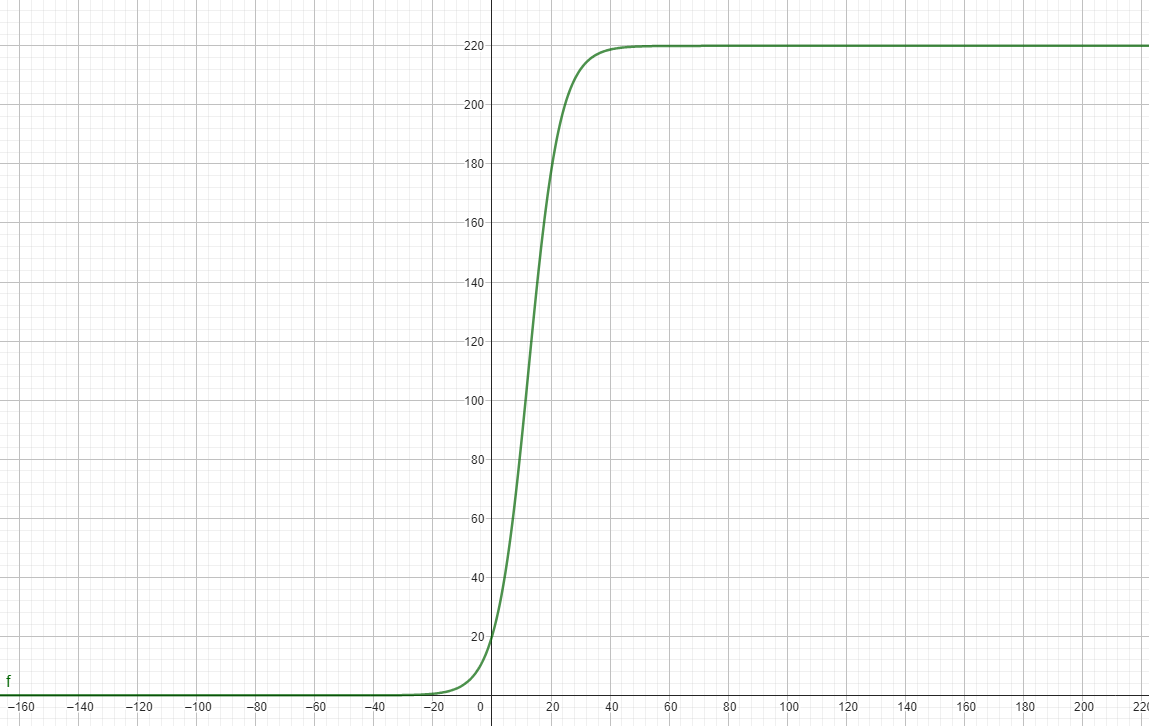
\includegraphics[width=0.6\textwidth]{matemáticas/Ejercicio13/grafica.png}
    \caption{Gráfica de la población de borregas en función del tiempo.}
    \end{figure}

    La gráfica muestra una curva de crecimiento logístico, típica de poblaciones con recursos limitados.

    **Cálculos y Resultados**

    Partimos de la ecuación:
    
    \[
    80 = \frac{220}{1 + 10 \cdot e^{-0.1863t}}
    \]
    
    Despejamos \( t \):
    
    \[
    80 \cdot \left(1 + 10 \cdot e^{-0.1863t}\right) = 220
    \]
    
    \[
    1 + 10 \cdot e^{-0.1863t} = \frac{220}{80}
    \]
    
    \[
    10 \cdot e^{-0.1863t} = \frac{220}{80} - 1
    \]
    
    \[
    e^{-0.1863t} = \frac{\frac{220}{80} - 1}{10}
    \]
    
    \[
    -0.1863t = \ln\left(\frac{\frac{220}{80} - 1}{10}\right)
    \]
    
    \[
    t = \frac{\ln\left(\frac{\frac{220}{80} - 1}{10}\right)}{-0.1863}
    \]
    
    Calculando \( t \), obtenemos que el tiempo mínimo necesario para que la población sea autosuficiente (es decir, alcance los 80 individuos) es aproximadamente 9.36 años. Esto confirma que el programa de repoblación debe durar al menos ese tiempo.
    
    \section*{c) Determinar la capacidad máxima de borregos que puede albergar el área protegida}
    
    Para encontrar la capacidad máxima, calculamos el límite de \( N(t) \) cuando \( t \) tiende a infinito:
    
    \[
    \lim_{t \to \infty} N(t) = \frac{220}{1 + 10 \cdot e^{-0.1863 \cdot \infty}}
    \]
    
    Dado que \( e^{-0.1863 \cdot \infty} \) tiende a cero, la expresión se simplifica a:
    
    \[
    \lim_{t \to \infty} N(t) = \frac{220}{1 + 0} = 220
    \]
    
    Esto significa que la capacidad máxima de borregos que puede albergar el área protegida es de 220 individuos.
    
    \section*{Resumen}
    
    \begin{itemize}
        \item \textbf{Tiempo mínimo para autosuficiencia}: Se necesitan al menos 9.36 años para que la población alcance los 80 individuos.
        \item \textbf{Capacidad máxima}: El área protegida puede albergar un máximo de 220 borregos cimarrones según el modelo.
    \end{itemize}
    **Conclusiones**
    La población de borregas sigue un patrón de crecimiento logístico, alcanzando una capacidad de carga de 220 individuos. El modelo matemático proporciona una herramienta útil para predecir el crecimiento de la población y tomar decisiones de manejo.

\end{document}